\section{Audio Equipment}
\subsection{Audio Signal Path}

\begin{figure*}[h]
\centering
\includegraphics[width=.85\textwidth]{Images/BlockDiagramAudio.png}
\caption{Block Diagram of Audio Signal Path}
\label{fig:fullfig}
\end{figure*}

\subsection{Line 6 TonePort MK2}

The audio interface for the MIDI Lab. Please do not change any parameters on the hardware or the supporting software. 

\subsection{DMV-Pro Effects Processor}

The DMV-Pro is the MIDI Lab's hardware effects processor with dual true-stereo inserts. To send audio to the effects processor, select the synth channel and pot the first two red auxiliary knobs. To change the parameters, rotate the three large black knobs on the effects processor.\\
\linebreak
\href{https://github.com/dkadyrov/MIDILab/blob/master/Manuals/DMV_Pro.pdf}{DMV-Pro Effects Processor Manual (PDF)}

\begin{figure*}[h]
\centering
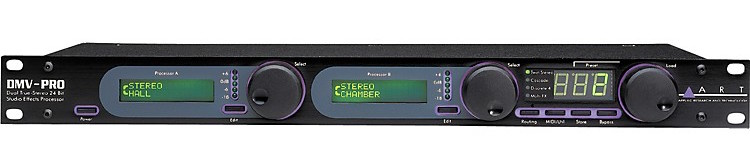
\includegraphics[width=.85\textwidth]{Images/DMVPRO.jpg}
\caption{DMV-PRO Effects Processor}
\label{fig:fullfig}
\end{figure*}

\newpage
\subsection{Mackie CR1604 VLZ Mixer}

16 channel audio mixer with ability to send audio to effects processor, other keyboards (for sampling), and for recording on the iMac as well as to a personal computer through a personal audio interface.\\
\linebreak
\href{https://github.com/dkadyrov/MIDILab/blob/master/Manuals/Mackie_Manual.pdf}{Mackie CR1604 VLZ Mixer Manual (PDF)}


\begin{figure}[h]
\centering
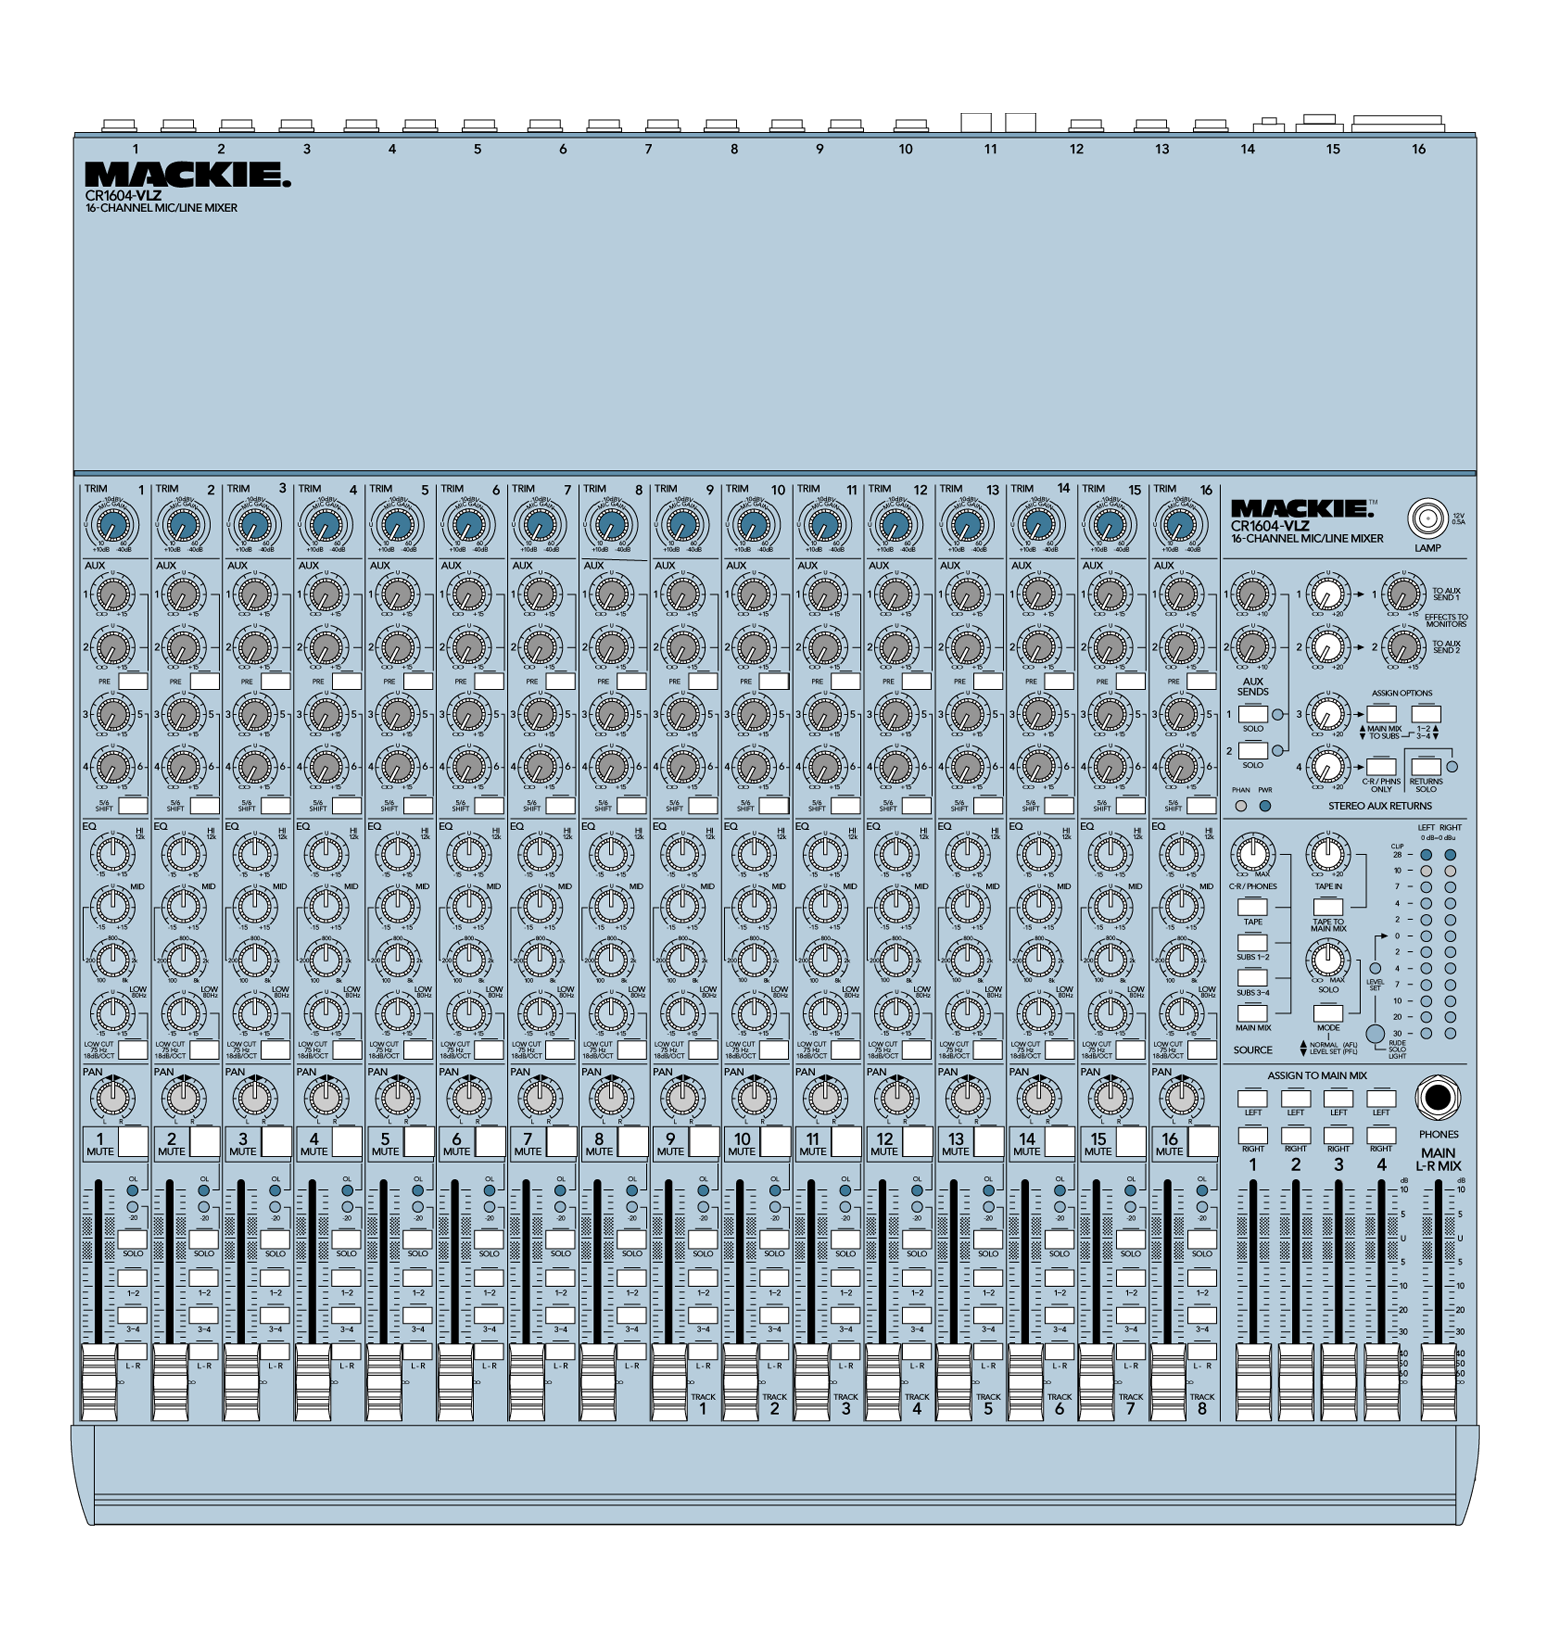
\includegraphics[width=.85\textwidth]{Images/Mackie_Manual-1.png}
\caption{Mackie CR1604 Mixer}
\end{figure}

\newpage

\subsubsection{Control of Individual Channel}

\begin{multicols}{2}
\small
\begin{enumerate}
	\item Volume Fader: Controls the volume of the channel within the mixer
	\item Path (Subs): Chooses where the channel signal is directed to
	\begin{enumerate}
		\item \textbf{Solo}: Isolates the channel in the mix. Useful for when you only want to hear the specific channel without other ones.
		\item \textbf{1-2}: Sends to Computer for Recording
		\item \textbf{3-4}: Sends to stereo $\frac{1}{4}$" cables for use with personal audio interfaces.
		\item \textbf{L-R}: Sends only to Monitors (Speakers)
	\end{enumerate}
	\item Mute: Mutes the Channel
	\item Pan: Controls the amount of signal sent to the left vs right, 1 vs 2, or 3 vs 4
	\item Equalization (EQ)
	\begin{enumerate}
		\item \textbf{High EQ}: $\pm 15$ dB at $12$ kHz
		\item \textbf{Mid EQ}: $\pm 15$ dB within 1.5 octaves of the frequency center (Determined by Frequency Sweep)
		\item \textbf{Frequency Sweep}: Selects the center of the Mid EQ between $100$ Hz and $8$ kHz
		%\item \textbf{Low EQ}: $\pm 15$ dB at $80$ Hz
		\item \textbf{Low Cut Switch}: Removes all signal below $75$ Hz (High Pass Filter)
	\end{enumerate}
	\item Auxiliary Sends: Sends a parallel signal path to other outputs on the mixer. See \ref{fig:signal} for more information.
	\begin{enumerate}
		\item \textbf{Aux A-B}: The DMV Pro effects processor has two inputs and can run different effects on each input. Aux \textbf{A} sends a signal to input 1 on the processor and Aux \textbf{B} sends a signal to input 2. See the section on the \hyperlink{effects processor}{effects processor}.
		\item \textbf{Aux C-D}: Not used
	\end{enumerate}
	\item Trim (Gain): Controls the amplitude of the signal going into the mixer. Input sensitivity is adjusted by $-10$ dB to $40$ dB. Please do not adjust unless necessary.
\end{enumerate}

\begin{center}
  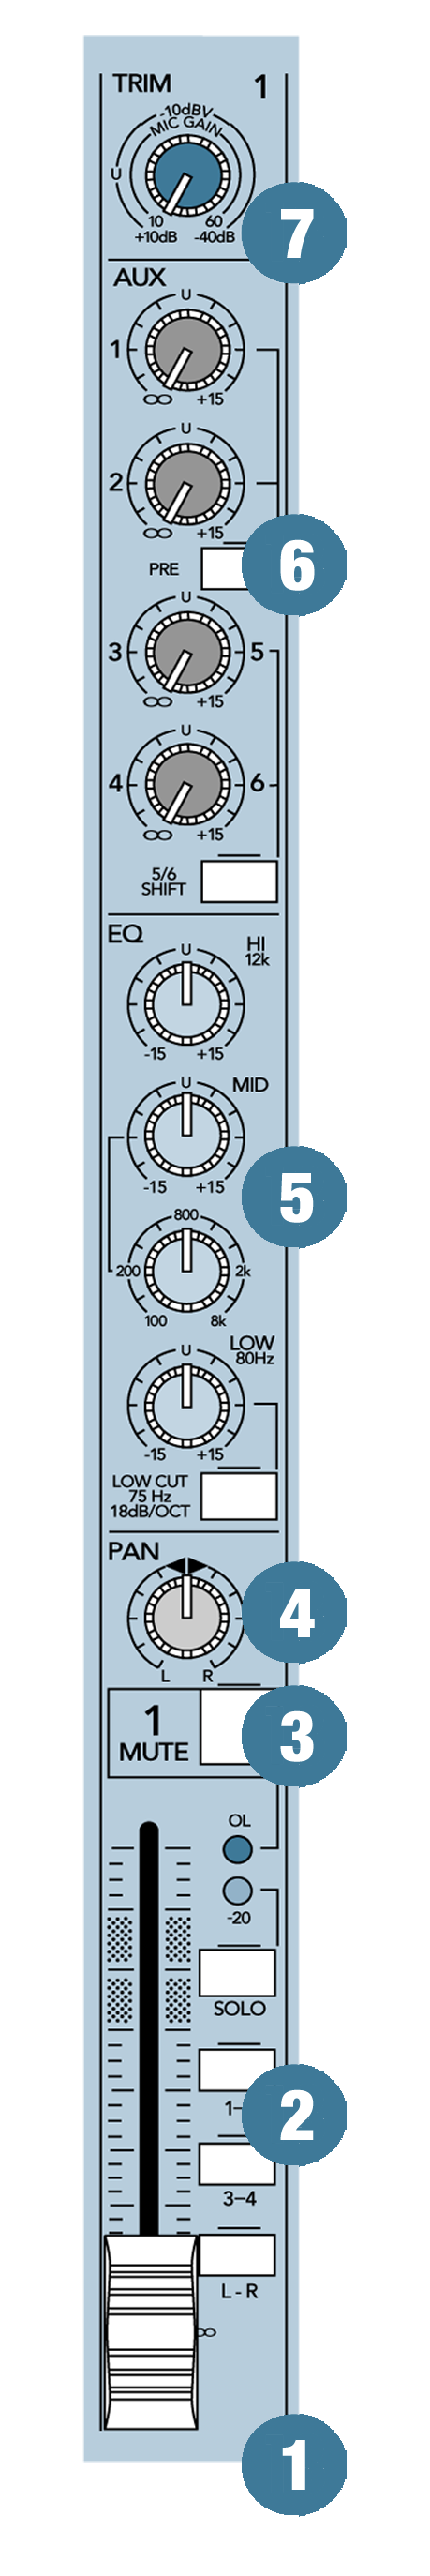
\includegraphics[height=220mm]{Images/Mackie.png}
  %\captionof{figure}{AA \cite{BB}}
\end{center}

\end{multicols}

\newpage

\subsubsection{Control of Mixer}
\begin{multicols}{2}
\small
\begin{enumerate}
	\item Effects to Monitors: Adds effects to monitors.
	\item Aux 1-2 Sends: Controls the gain of the AUX 1-2 send output into the mixer.
	\item AUX Returns: Controls the volume of the signal returning from the AUX within the mixer.
	\item 1-2/3-4 Toggles: Controls the path of the signal to
	\item IGNORE ABOVE
	\item C-R/Phones: Controls volume to the Control Room out and the Headphone Jack
	\item Selects what inputs are routed to the meter display
	\item Meter Display: Visually shows the strength of the signal. Want the highest possible signal strength (green) without clipping (red light). At yellow compression occurs.
	\item Selects what inputs are routed to the meter display, the C-R out and the headphone jack.
	\item Solo Knob: Controls the level of the soloed channels
	\item Mode Control:
	\begin{enumerate}
		\item \textbf{Normal (AFL)}: solo signal is post EQ, Pan, and Fader
		\item \textbf{Level Set (PFL)}: solo signal is pre EQ, Pan, and Fader
	\end{enumerate}
	\item \hypertarget{Headphone Jack}{Headphone Jack}: Accepts $\frac{1}{4}$ in. plug. Feel free to use your own headphones.
	\item Main Mix Assigns: Allows fader subgroups 1-4 to be assigned left, right, or both channels in main mix.
	\item Subgroup Volume Faders: Control the output levels of chosen group. Adjusting the volume of subgroup 1-2 will change the volume audio into the iMac. Adjusting 3-4 will change volume of the audio going into personal audio equipment.
	\item Master Fader: controls output to speakers.
\end{enumerate}
\begin{center}
  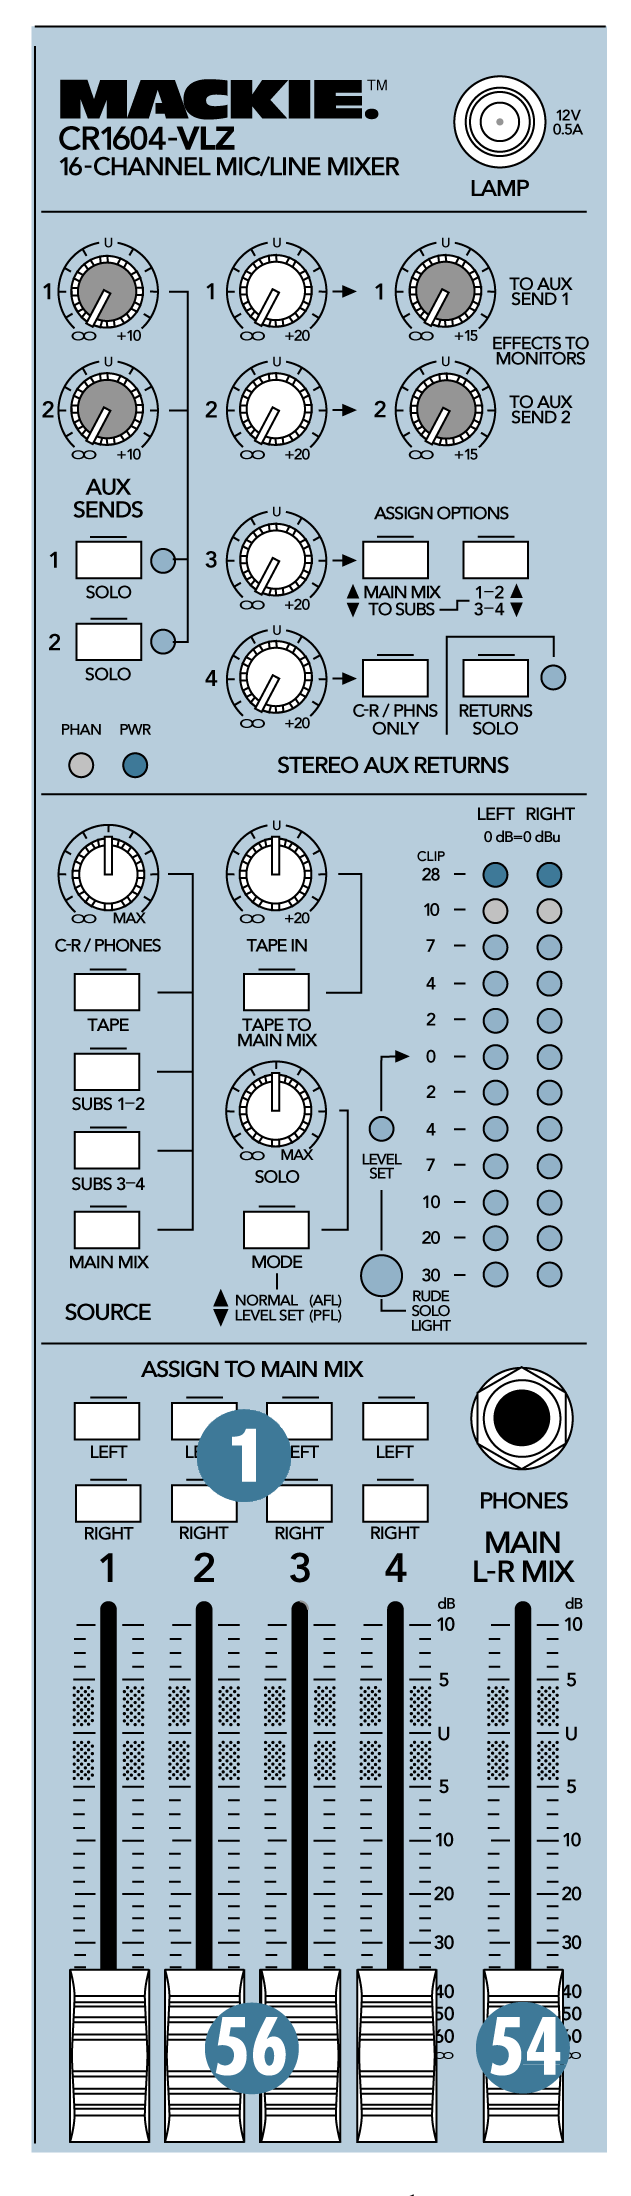
\includegraphics[height=220mm]{Images/Mackie_2.png}
  %\captionof{figure}{AA \cite{BB}}
\end{center}
\end{multicols}


